\section{Leseger"ate und -verfahren}
In diesem Kapitel sollen verschiedene Lesegeräte und ihre Anwendungsszenarien kurz vorgestellt werden.

\subsection{Handleser}
Bei den Handlesern gibt es verschiedene Funktionsweisen. Zum einen der \textbf{CCD-Handleser} für 1D-Codes. CCD steht für "Charged Coupled Device" (dt. \textit{ladungsgekoppeltes Bauteil}) und bezieht sich auf den eingebauten Sensor, der ein ebensolcher ist. CCD-Sensoren sind lichtempfindliche, elektronische Bauelemente, die auf dem inneren Photoeffekt beruhen\footnote{Zur näheren Funktionsweise des CCD-Sensors siehe zum Beispiel \url{http://www.ccd-sensor.de/}}. der CCD-Handleser ist im Prinzip aufgebaut wie eine Strichcode-Kamera mit CCD-Zeile. Da der Code mit ausreichend Kontrast auf dem Sensor abgebildet werden muss, muss er beleuchtet werden. Da eine Lichtquelle mit zunehmendem Abstand vom Sensor immer weniger Licht zur Umgebung hinzufügt, hat der CCD-Handleser einen Maximalabstand zum Code in Abhängigkeit zur Größe des Codes. Hinsichtlich der Neigung und Drehung ist der Handleser recht tolerant, sodass er auch bei einer Neigung von bis zu $\pm65^\circ$ zur Senkrechten und einer Drehung von bis zu $\pm80^\circ$ zur Senkrechten einen Barcode problemlos lesen kann (siehe dazu auch Abbildung~\ref{fig:neigungswinkel} und Abbildung~\ref{fig:drehwinkel}). CCD-Handleser werden mit integrierten Decodern gebaut und können über eine Vielzahl von Schnittstellen an bestehende Systeme angeschlossen werden, z.B. über USB, OCR, Tastaturemulation, \dots \\

\begin{figure}[htbp]
	\parbox{.47\textwidth}{\centering
		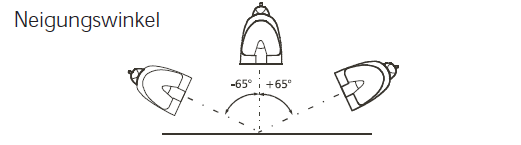
\includegraphics[height=2.5cm]{Bilder/Neigungswinkel.png}
		\caption{Neigungswinkel}
		\label{fig:neigungswinkel}}
	\hfill
	\parbox{.47\textwidth}{\centering
		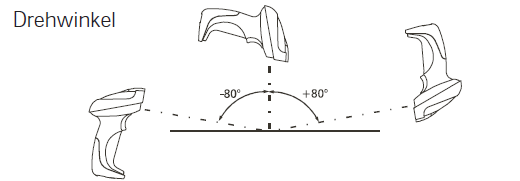
\includegraphics[height=2.5cm]{Bilder/Drehwinkel.png}
		\caption{Drehwinkel}
		\label{fig:drehwinkel}}
	\hfill
\end{figure}

Ein weiterer Leser für 1D-Codes ist der \textbf{Handscanner auf Laserbasis}. Sein Leseprinzip ist von dem eines Laserscanners abgeleitet. Eingebaut ist in ihm eine Laserdiode, die einen Laserstrahl erzeugt, welcher über einen Schwingspiegel abgelenkt wird. Dadurch entsteht in der Leseebene ein wandernder Lichtfleck, der den Strichcode abtastet. Insgesamt erlaubt dieser Handscanner eine größere Distanz als der CCD-Handleser, jedoch ist er im Drehwinkel nicht ganz so tolerant (nur $\pm60^\circ$ zur Senkrechten). Er kann ebenfalls über eine Vielzahl von Schnittstellen an bestehende Systeme angebunden werden.

Der \textbf{2D-Leser}

\subsection{loremsub}
Lorem ipsum dolor sit amet, consetetur sadipscing elitr, sed diam nonumy eirmod tempor invidunt ut labore et dolore magna aliquyam erat, sed diam voluptua. At vero eos et accusam et justo duo dolores et ea rebum. Stet clita kasd gubergren, no sea takimata sanctus est Lorem ipsum dolor sit amet. Lorem ipsum dolor sit amet, consetetur sadipscing elitr, sed diam nonumy eirmod tempor invidunt ut labore et dolore magna aliquyam erat, sed diam voluptua. At vero eos et accusam et justo duo dolores et ea rebum. Stet clita kasd gubergren, no sea takimata sanctus est Lorem ipsum dolor sit amet.
\pagebreak
